\documentclass[a4,12pt]{scrartcl}

%Basic 
\usepackage[utf8]{inputenc}
\usepackage[ngerman]{babel}
\usepackage[T1]{fontenc}
%Schrift 
\usepackage{textcomp} % Für μ \textmu
%\usepackage{fontspec} 
%\setmainfont{Arial} 
%Zeilenabstand
\usepackage{setspace}
\setstretch {1.3}
\usepackage{float}
\usepackage[bottom = 3.50cm]{geometry}

%Titel Seite
\usepackage{titling} %Wird benötigt damit \maketitle die Variabeln title, author und date nicht überschreibt
\title{Software Architektur}
\subtitle{Projekt: sniffdatel}
\author{David Meister \and Giorgio Vincenti \and Samuel Krieg \and Andreas Stalder}		
 %mit /and können Personen hinzugefügt werden
\date{\today}


%Kopf, Fusszeile
\usepackage{fancyhdr}
\pagestyle{fancy}
\lhead{SW Engineering Projekt FS 2016}
\chead{}
\rhead{sniffdatel}
\lfoot{\thetitle \: v1.1 }
\cfoot{\today }
\rfoot{Seite \thepage}
\renewcommand{\headrulewidth}{0.4pt}

%Bilder
\usepackage{graphicx}

%Zeichnen
\usepackage{tikz}

%Tabellen
\usepackage{booktabs}
\usepackage{longtable}

%Codesnippets
\usepackage{listings}
\lstset{language=java,basicstyle=\footnotesize,frame=single} %backgroundcolor=\color{lightgray}

%Querformat für eine Seite
\usepackage{lscape}
\usepackage{rotating}
\usepackage{pdflscape}

%URL 
\usepackage[colorlinks=true, linkcolor=blue, urlcolor=blue, citecolor=blue]{hyperref}
\urlstyle{same} 


%Loremimpsum
\usepackage{lipsum}



\begin{document}

%\clearpage\maketitle
\begin{titlepage}
	\centering
	\vspace{5cm}
	\begin{center}
	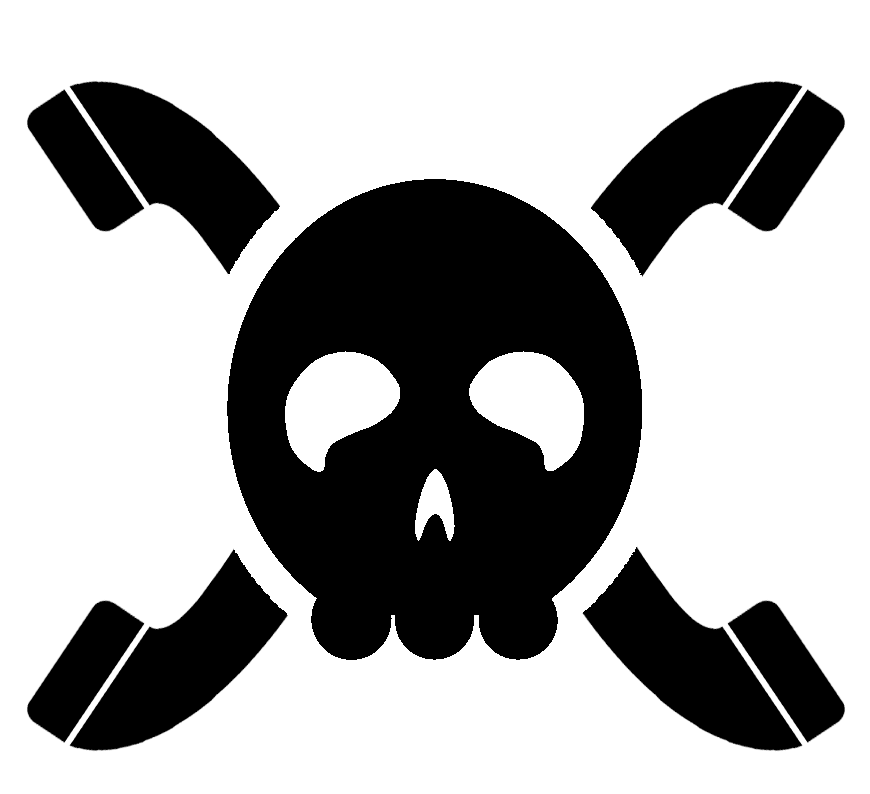
\includegraphics[width=0.50\textwidth]{logo.png}
	\end{center}
	{\huge\bfseries sniffdatel\par}
	\vspace{8cm}
	\raggedright
	{\bfseries SW Engineering Projekt FS 2016\par}
	{\huge\bfseries Software Architektur\par}
	\vspace{1cm}
	{\theauthor \par}
	{\today\par}

\end{titlepage}

\section{Änderungsgeschichte}

\begin{table}[htb]
\centering
    \begin{tabular}{@{} l l l l@{}}\toprule    
    {Datum} & {Version} & {Änderung} & {Autor}\\ \midrule
    15.03.16 & 0.9 & Erstellung erster Version & Giorgio Vincenti\\ \addlinespace
    18.04.16 & 1.0 & Review ready & alle\\
    26.04.16 & 1.1 & Korrektur & alle\\ \addlinespace
    \bottomrule
    \end{tabular}
\caption{\textbf{Änderungsgeschichte}}
\end{table}
\newpage
%\thispagestyle{empty}
\tableofcontents
\newpage

\section{Einführung}
\subsection{Zweck}
In diesem Dokument wird die Architektur von \textbf{sniffdatel} erläutert. Es soll als Wegweiser dienen und Hilfestellung  für die Entwicklung bieten.     
\subsection{Gültigkeitsbereich}
Das Dokument bezieht sich auf die Software \textbf{sniffdatel}, welche im Rahmen des Moduls Engineeringprojekt des Frühjahrssemester 2016 entwickelt wird und ist während des gesamten Projekts gültig. 
\subsection{Referenzen}
\begin{itemize}
\item doc/02\_projektplan/Projektplan\_v1.2
\item doc/03\_analyse/Anforderungsspezifikationen\_v1.0
\item doc/03\_analyse/Domainanalyse\_v1.0
\item doc/04\_architektur/externes\_design\_v1.0
\end{itemize}
Diese Dokumente sind bei uns auf der Dropbox oder auf Github zu finden. Für den Betreuer sind die Dokumente auf Redmine vorhanden. 

\section{Systemübersicht}
In der nachfolgenden Abbildung ist eine Darstellung des Systems ersichtlich. Die Applikation lässt sich auf einer beliebigen Linux Distribution mit installiertem JRE (Java Runtime Environment) ab Version 8 starten. Über das GUI wird der Packet Scanner gestartet. Der Packet Scanner wir mit der jnet pcap - und das GUI mit der JavaFX Library realisiert. Die Applikation hat eine eigene Filterlogik implementiert um Sessions zu finden, anzuzeigen und die dazugehörigen RTP Pakete weiter zu verarbeiten. Die RTP Payloads werden in einen Buffer geschrieben und der Audioplayer (javax.sound Library) spielt den RTP Payload ab.
\begin{figure} [H]
	\begin{center}
	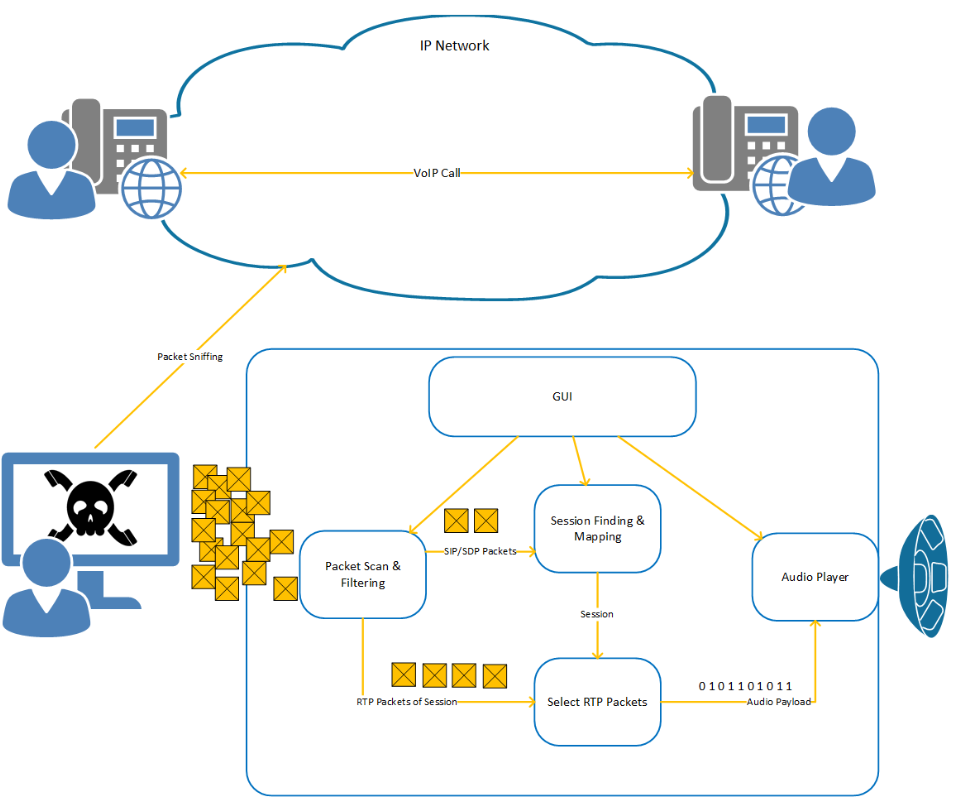
\includegraphics[width=0.90\textwidth]{./pictures/systemubersicht.PNG}

	\label{Bild Referenz}
	\end{center}
\end{figure}
\section{Architektonische Ziele und Einschränkungen}

\subsection{Ziele}
\begin{itemize}
\item Die Software soll benutzerfreundlich gestaltet werden. Es sollte jedem möglich sein, ohne grosses Know-How, ein VoIP Gespräch im Netzwerk abzuhören. 
\item Die Software sollte von einem beliebigen Linux Client gestartet und genutzt werden können. 
\item Die Benutzeroberfläche der Software soll einfach und übersichtlich gestaltet sein.
\end{itemize}
\subsection{Einschränkungen}
\begin{itemize}
\item Die Software muss auf den Clients als Administrator ausgeführt werden, damit der Zugriff auf die Netzwerkschnittstellen sauber funktioniert. 
\item Die Software kann keine verschlüsselten Pakete wiedergeben. 
\item Das Abspielen eines Gesprächs benötigt eine gewisse Zeit um die gesammelten RTP Pakete zwischenzuspeichern und abzuspielen. Es wird mit einer Verzögerung von maximal einer  Sekunde gerechnet.
\item Die Software kann nur neu eingehende VoIP Anrufe erkennen (Verbindungsaufbau muss mitgeschnitten sein) und als Session im GUI anzeigen. RTP Pakete ohne zugehörenden Verbindungsaufbau (SIP & SDP) könen nicht detektiert werden. 
\item Es kann nur der G.711(\textmu -law/A-law) Codec abgespielt werden.
\item Die Software beschränkt sich auf UDP-Verkehr und erkennt somit Gespräche welche TCP involvieren nicht.
\item Die Software wird nur unter Linux Distributionen unterstützt.
\end{itemize}
\subsection{Tools}
\begin{description}
\item [astah:] Werkzeugtool für das modellieren von Diagrammen während dem gesamten Projekt.
\item [Eclipse:] Entwicklungsumgebung für die Software.
\item [Java 8:] Es wird mit Java 8 entwickelt. 
\item [Texmaker:] Alle Dokumente rund ums Projekt werden mit Texmaker erstellt. 
\item [Jnetpcap:] Library um auf Netzwerkfunktionen zuzugreifen. Diese Library funktioniert nur unter Linux und Windows. Sie wird verwendet um auf die Netzwerkinterfaces eines Rechners zuzugreifen und um Netzwerkpakete zu sammeln.
\item [Javax.sound] Javax standard Sound Library.
\item [JUnit4:] Framework für Softwaretests.
\item [Eclemma:] Werkzeug im Eclipse für die Überprüfung der Codeabdeckung von Softwaretests. 
\item [e(fx)clipse:] JavaFX plugin für Eclipse
\item [Scene Builder 8.0:] Dieses Tool wird verwendet um das GUI zu erstellen. 
\item [Travis CI:] Tool für continuous integration.
\end{description}

\section{Logische Architektur}
\begin{figure} [H]
	\begin{center}
	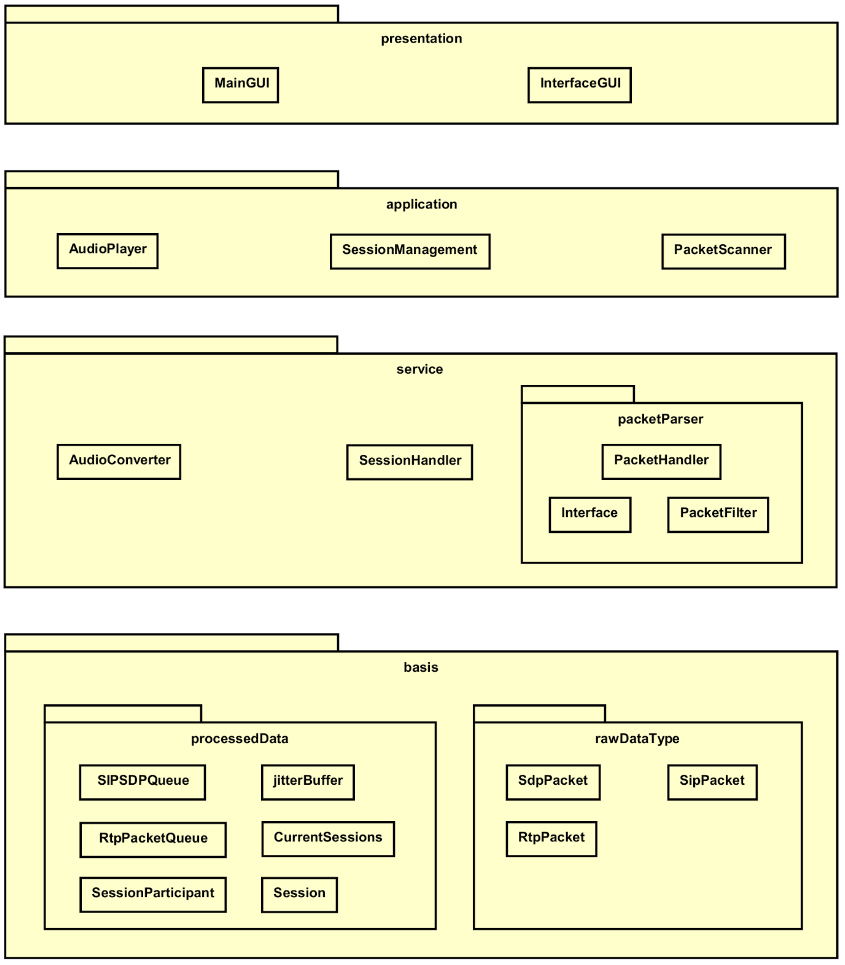
\includegraphics[width=0.90\textwidth]{./pictures/logischearchitektur1.PNG}
	\label{Bild Referenz}
	\end{center}
\end{figure}
\begin{figure} [H]
	\begin{center}
	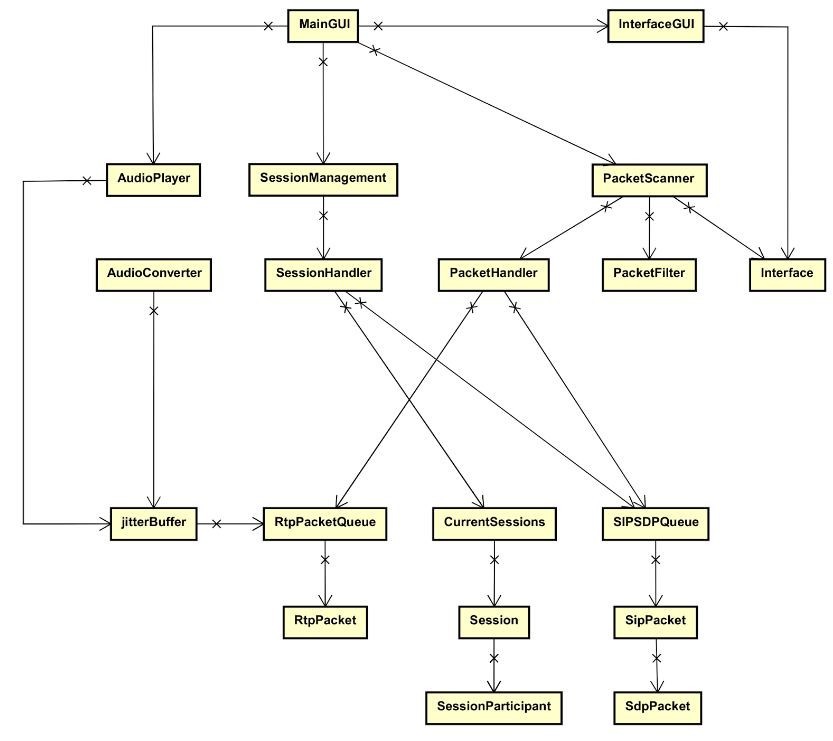
\includegraphics[width=0.90\textwidth]{./pictures/logischearchitektur2.PNG}
	\label{Bild Referenz}
	\end{center}
\end{figure}
\subsection{Presentation-Layer}
Im Präsentation-Layer wird eine MVC (Model, View, Control) Architektur verwendet. So kann das Design von der Logik getrennt werden. Dies bringt den Vorteil, dass zum Beispiel die View ausgetauscht werden kann, ohne dass man etwas an der Logik ändern muss.
\subsubsection{Klassenstruktur}

\begin{table}[H]
\centering
    \begin{tabular}{@{}l p{11cm} @{}}\toprule    
    {Klassenname} & {Beschreibung}\\ \midrule
    MainGUI & Das MainGUI ist die Hauptoberfläche. Von dieser aus wird alles gestartet und eingestellt. Diese Oberfläche führt auch zum InterfaceGUI. \\ \addlinespace
        InterfaceGUI & Im InterfaceGUI werden alle Interfaces angezeigt und man kann das gewünschte Interface bestimmen, auf dem der PacketScanner läuft. \\
    \bottomrule
    \end{tabular}
\end{table}
\subsubsection{Schnittstellen}
Der Presentation-Layer hat eine Schnittstelle zum Application-Layer, sowie zum Service-Layer. 
Das MainGUI hat eine Schnittstelle zum AudioPlayer, um diesen mittels GUI-Button zu starten und zu stoppen.
Zusätzlich besteht noch eine Schnittstelle zum SessionManagement, um die Session zu verwalten.
Eine weitere Schnittstelle besteht zum PacketScanner, damit dieser gesteuert werden kann, sowie zum InterfaceGUI.
Das InterfaceGUI hat eine Schnittstelle zum packetParser Package, welches sich auf dem Service-Layer befindet. Durch diese Schnittstelle kann das aktuelle Interface verwaltet werden.

\subsection{Application-Layer}
Der Application-Layer beinhaltet die grundlegenden Steuerungsklassen. Durch diesen Layer wird zum Beispiel der AudioPlayer gestartet und gestoppt
\subsubsection{Klassenstruktur}
\begin{table}[H]
\centering
    \begin{tabular}{@{}l p{10cm} @{}}\toprule    
    {Klassenname} & {Beschreibung}\\ \midrule
     PacketScanner& Der PacketScanner holt alle Pakete vom gewähltem Interface und übergibt diese dem PacketHandler. \\ \addlinespace
    AudioPlayer& Der AudioPlayer liest den 
    Buffer aus und spielt diesen Inhalt ab. Dabei gibt wird immer wieder überprüft ob der Buffer bereit ist, damit kein Over- oder Underflow entsteht. \\ \addlinespace
    SessionManagement&  Mit dem SessionManagement wird die aktuelle Session gesetzt, angepasst und verwaltet.\\ 
     
    \bottomrule
    \end{tabular}
\end{table}
\subsubsection{Schnittstellen}
Der Application-Layer greift auf den Service-Layer  und auf den Basis-Layer zu. Dieser beinhaltet alle Logikklassen, welche die Pakete verarbeitet und die Sessions erstellt, sowie die zwischengespeicherten Daten.
Der PacketScanner greift auf das Package packetParser zu, um die gesnifften Pakete zu verarbeiten.
Der AudioPlayer greifft auf den JitterBuffer zu, welche den zu abspielenden Payload beinhaltet.
Das SessionManagement greift auf den SessionHandler zu, um die aktuelle Session zu bearbeiten.

\subsection{Service-Layer}
Die Zuständigkeiten des Service Layers liegen in der Verarbeitung und Erstellung der vom Basis Layer zur Verfügung gestellten Daten.
\subsubsection{Packagestruktur}
\begin{table}[H]
\centering
    \begin{tabular}{@{}l p{11cm} @{}}\toprule    
    {Klassenname} & {Beschreibung}\\ \midrule
     packetParser& 
Das packetParser Package beinhaltet den PacketHandler, die Interfaceklasse, sowie den PacketFilter. \\ 
    \bottomrule
    \end{tabular}
\end{table} 
\subsubsection{Klassenstruktur}
\begin{table}[H]
\centering
    \begin{tabular}{@{}l p{11cm} @{}}\toprule    
    {Klassenname} & {Beschreibung}\\ \midrule
     AudioConverter& Der AudioConverter verarbeitet den Audio Payload zu einem abspielbaren Byte Array und füllt dieses in den jitter Buffer. \\ \addlinespace
        SessionHandler  & Der SessionHandler holt die SIP und SDP Pakete aus der SIPSDPQueue und verarbeitet diese zu neuen Sessions. Falls die Session bereits besteht, wird die richtige Session angepasst. \\ 
    \bottomrule
    \end{tabular}
\end{table}
\subsubsection{Schnittstellen}
Der Service hat eine Schnittstelle zum Basis-Layer, welche die Datenstruktur beinhaltet. Der SessionHandler hat eine Schnittstelle zum processedData Package, wo die neuen Sessions gespeichert werden, sowie die vorhandenen angepasst werden.
Die Schnittstellen des AudioConverters sind auf dem processedData Package. Der AudioConverter holt die Pakete aud der RtpPacketQueue, verarbeitet diese und schreibt den Payload in den JitterBuffer.

\subsection{PacketParser-Package}
\subsubsection{Klassenstruktur}
\begin{table}[H]
\centering
    \begin{tabular}{@{}l p{11cm} @{}}\toprule    
    {Klassenname} & {Beschreibung}\\ \midrule
     PacketHandler& 
Der PacketHandler beinhaltet die Paketlogik. Hier wird jedes Paket überprüft und falls dies ein SIP, SDP oder ein RTP Paket ist, wird es in eine Liste auf dem unteren Layer gespeichert.
 \\ \addlinespace
     Interface&  
Die Klasse Interface steuert die Interfaceanzeige und Auswahl. Hier werden alle vom Betriebssystem vorhandenen Interface gespeichert und und das aktuell gewünschte Interface gesetzt.
\\ \addlinespace
     PacketFilter&  
Im PacketFilter wird der Filter gesetzt, welche Pakete vom PacketScanner bearbeitet werden sollen. In unserem Fall wird hier alles herausgefiltert, was nicht ein UDP-Paket ist.
\\ 
    
    \bottomrule
    \end{tabular}
\end{table}
\subsubsection{Schnittstellen}
Das parserPacket Package hat eine Schnittstelle zum rawDataType und processedData Package, um die Daten in den Queues zwischenzuspeichern.

\subsection{Basis-Layer}
Die “basis” Schicht beinhaltet die zu verarbeitenden Daten. Höhere Schichten lesen und schreiben in- und von der basis Schicht aufgrund ihrer eigens definierten Logik. 
\subsubsection{Klassenstruktur}
\begin{table}[H]
\centering
    \begin{tabular}{@{}l p{11cm} @{}}\toprule    
    {Package Name} & {Beschreibung}\\ \midrule
     processedData& Das Package “processed Data” stellt den höher liegenden Schichten die benötigten Daten über fertige Datenstrukturen (Queue, Lists, etc.) zur Verfügung. \\ \addlinespace
     rawDataType& Im Package “rawDataType” sind die Implementationen der benötigten Datenpakete. Diese Objekte werden für die Weiterverarbeitung in den höheren Schichten verwendet. \\ 
    \bottomrule
    \end{tabular}
\end{table}
\subsubsection{Schnittstellen}
Hier bestehen keine Schnittstellen.

\subsection{processedData-Package}
Das Package “processed Data” stellt den höher liegenden Schichten die benötigten Daten über fertige Datenstrukturen (Queue, Lists, etc.) zur Verfügung. 
\subsubsection{Klassenstruktur}
\begin{table}[H]
\centering
    \begin{tabular}{@{}l p{11cm} @{}}\toprule    
    {Klassenname} & {Beschreibung}\\ \midrule
     Session&  
Das Sessionobjekt beinhaltet Informationen über die Session (Methoden, Teilnehmer)
\\ \addlinespace
     SessionParticipant & 
Das SessionParticipant Objekt beinhaltet die IP-Adresse, SIP-URI und Port
 \\ \addlinespace
       CurrentSessions& 
Das CurrentSession Objekt speichert die gefundenen Sessions
 \\ \addlinespace
       RtpPacketQueue & 
Die RtpPacketQueue beinhaltet die zu verarbeitenden RTP Pakete
 \\ \addlinespace
       SIPSDPQueue  &  
Die SIPSDPQueue beinhaltet die zu verarbeitenden SIP/SDP Pakete
\\ \addlinespace
        JitterBuffer  & 
Der Jitter Buffer beinhaltet den fertigen Audio Payload
 \\ 
    \bottomrule
    \end{tabular}
\end{table}
\subsubsection{Schnittstellen}
Hier bestehen keine Schnittstellen.

\subsection{RawDataType-Package}
Im Package “rawDataType” sind die Implementationen der benötigten Datenpakete. Diese Objekte werden für die Weiterverarbeitung in den höheren Schichten verwendet.

\subsubsection{Klassenstruktur}
\begin{table}[H]
\centering
    \begin{tabular}{@{}l p{11cm} @{}}\toprule    
    {Klassenname} & {Beschreibung}\\ \midrule
     SipPacket& 
Dieses Objekt beinhaltet Informationen (z.B. Source, Destination, CallID etc.) über das VoIP Gespräch
 \\ \addlinespace
       SdpPacket   & 
Wird verwendet um Informationen (Ports, Codecs) für die Session zu gewinnen
 \\ \addlinespace
        RtpPacket       & 
Dieses Objekt beinhaltet neben dem Payload noch die Attribute ssrc, seqNr, timeStamp und Port 
 \\ 
    \bottomrule
    \end{tabular}
\end{table}
\subsubsection{Schnittstellen}
Hier bestehen keine Schnittstellen.



\section{Prozesse und Threads}
Die Funktionalität der Software macht Parallelität notwendig. Es ist zum Beispiel nicht möglich, dass der Audioplayer mit dem Abspielen des RTP Payloads wartet, bis der Scanner terminiert. Wir setzen auf Multithreading, um den Anforderungen gerecht zu werden.
\subsection{Prozesse}
Beim Ausführen eines Java Programms wird eine Java Virtual Machine (JVM) gestartet. Die JVM läuft auf einem einzelnen Prozess im Betriebssystem. 
\subsection{Threads}
Beim Ausführen eines Java Programms ruft ein neu erzeugter Thread die main() - Methode auf. Über die main() - Methode starten wir in einem eigenen Thread das GUI. Weitere für die Programmausführung notwendige Threads werden vom GUI-Thread gestartet. Die Threadumschaltung resp. das Scheduling wird von der JVM selbst übernommen.
\subsubsection{Datenstrukturen}
Um die Daten zwischenzuspeichern, werden Threadsichere Datenstrukturen verwendet. Dies ist zum Beispiel beim Jitter-Buffer eine ConcurrentLinkedQueue und bei allen anderen Queues eine TransferQueue. Diese sind alle schon in der Standard Java Library vorhanden.
\subsubsection{Thread Model}
\begin{figure} [H]
	\begin{center}
\begin{verbatim}
main()
  |
  |
  |---------guiThread()
  |            |
  |            |
  |            |-----scannerThread()
  |            |            |
  |            |            |
  |            |------------------sessionThread() und converterThread()
  |            |            |            |
  |            |            |            |
  |            |---------------------------------audioThread()
  |            |            |            |            |
  |            |            |            |            |
  |            |            |            |            |
  |            |            |            |            |
  |            |            |            |            |
  |            |            |            |            |
  |            |            |            |            |
  |            |            |            |            |
  |            |            |            |            |
  |            |            |            |            |
\end{verbatim}
\end{center}
\end{figure}

\section{Datensicherung}
Sniffdatel kommt ohne persistente Datenspeicherung aus. Transistente Daten wie aktuell im Neztwerklaufende VoIP-Session  mit den zugehörigen VoIP-Teilnehmern werden in Datenstrukturen gepuffert.
\subsection{Jitter-Buffer}
Bei der Übertragung von VOIP-Datenpaketen gibt es gewisse Verzögerungen im Netzwerk. Diese Verzögerungen können sehr unterschiedlich sein und werden als Jitter und Delay bezeichnet. Diese Verzögerungen führen zu einer schlechteren Sprachqualität. Um dies zu vermeiden, greift man auf einen Jitter-Buffer zurück. Dieser speichert den eingehenden Verkehr, um gleichmässigen Datenfluss zu garantieren. 
Mit dem Jitter-Buffer werden vier Probleme behoben. Den Jitter, Packet loss und Out-Of-Order.
\subsubsection{Delay}
Netzwerkpakete können durch hohe Last auf dem Netzwerk verzögert werden. Dadurch entsteht Delay (Verzögerung). Um diese Verzögerung zu korrigieren, wird der Jitter-Buffer eingesetzt. Dieser puffert die Daten für eine Sekunde in der Queue, damit sicher genügend Pakete vorhanden sind.
\subsubsection{Jitter}
Jitter ist eigentlich sehr änhnlich wie der Delay. Es handelt sich nur im einen variablen Delay. Somit können wir auch diese Verzögerung mit dem Jitter-Buffer entfernen.
\subsubsection{Packet loss}
Da Pakete auf dem Weg zum Empfänger verloren gehen können, muss der Packet loss beachtet werden. Fehlen mehr als 1\% der Pakete, verschlächtert sich die Soundqualität.
Der Packet loss kann sehr leicht durch die Sequenznummer erkannt werden.
Um die fehlenden Pakete zu korrigieren, werden durch den AudioConverter 'Null Pakete' hinzugefügt. Diese Pakete enthalten nur Null Bytes und werden vom Player lautlos abgespielt.
Dies ist aber ein optinales Feature.
\subsubsection{Out-Of-Order}
Pakete können aus der Reihenfolge kommen, was die Audioqualität beinträchtigt.
Mit Sniffdatel werden als ersten Schritt, die später eintreffenden Pakete verworfen, um die Soundqualität zu steigern. Ein optinales Feature wird sein, die Paketreihenfolge mit dem Jitter-Buffer wiederherzustellen. Dabei wird die Sequenznummer und der Timestamp verwendet.
\subsubsection{Datenstruktur}
Als Datenstruktur wird eine ConcurrentLinkedQueue verwendet. Diese ist Threadsicher und kann somit von meheren Thread (AudioPlayer, AudioConverter) bearbeitet werden. 

\section{Grössen und Leistungen}
\subsection{Leistung}
Sniffdatel wird auf eine Datenrate von 100Mbit/s beschränkt. Die Software sollte auf jedem beliebigen Netzwerk, mit der erwähnten Datenrate funktionieren. Der Buffer sowie die Parallelisierung wird dementsprechend integriert. 
\subsection{Anzahl Sessions}
Sniffdatel wird betreffend den anzuzeigenden Sessions auf maximal 50’000 beschränkt. Diese Beschränkung ist nicht kritisch für Sniffdatel, da diese nur temporär in einer Liste gespeichert sind.
\subsection{Verzögerung}
Als maximale Verzögerung legen wir eine Sekunde fest. Diese Verzögerung betrifft das Zwischenpuffern, damit die Audiodaten flüssig abgespielt werden können.
\subsection{Buffergrösse}
Sniffdatel kann audio mit dem Codec G.711(\textmu -law/A-law) wiedergeben. Da dieser Codec mit einer Datenübertragungsrate von 8000Hz*8Bit funktioniert, wird die Grösse des Jitter-Buffers auf 8KByte (64Kbit/8) festgelegt. Dies entspricht einer Sekunde. 
\end{document}

